\let\negmedspace\undefined
\let\negthickspace\undefined
\documentclass[journal,12pt,onecolumn]{IEEEtran}
\usepackage{cite}
\usepackage{amsmath,amssymb,amsfonts,amsthm}
\usepackage{algorithmic}
\usepackage{graphicx}
\graphicspath{{./figs/}}
\usepackage{textcomp}
\usepackage{xcolor}
\usepackage{txfonts}
\usepackage{listings}
\usepackage{enumitem}
\usepackage{mathtools}
\usepackage{gensymb}
\usepackage{comment}
\usepackage{caption}
\usepackage[breaklinks=true]{hyperref}
\usepackage{tkz-euclide} 
\usepackage{listings}
\usepackage{gvv}                                        
%\def\inputGnumericTable{}                                 
\usepackage[latin1]{inputenc}     
\usepackage{xparse}
\usepackage{color}                                            
\usepackage{array}
\usepackage{longtable}                                       
\usepackage{calc}                                             
\usepackage{multirow}
\usepackage{multicol}
\usepackage{hhline}                                           
\usepackage{ifthen}                                           
\usepackage{lscape}
\usepackage{tabularx}
\usepackage{array}
\usepackage{float}
\newtheorem{theorem}{Theorem}[section]
\newtheorem{problem}{Problem}
\newtheorem{proposition}{Proposition}[section]
\newtheorem{lemma}{Lemma}[section]
\newtheorem{corollary}[theorem]{Corollary}
\newtheorem{example}{Example}[section]
\newtheorem{definition}[problem]{Definition}
\newcommand{\BEQA}{\begin{eqnarray}}
\newcommand{\EEQA}{\end{eqnarray}}
\newcommand{\define}{\stackrel{\triangle}{=}}
\theoremstyle{remark}
\newtheorem{rem}{Remark}

\begin{document}

\title{12.173}
\author{ee25btech11056 - Suraj.N}
\maketitle
\renewcommand{\thefigure}{\theenumi}
\renewcommand{\thetable}{\theenumi}

\begin{document}

\textbf{Question :} Consider the system \\

\[
\begin{aligned}
x + 10y &= 5 \\
y + 5z  &= 1 \\
10x - y + z &= 0
\end{aligned}
\]

On applying \textbf{Gauss-Seidel} method , x correct up to 4 decimal places is

\textbf{Solution :}

\begin{table}[h!]
  \centering
  \begin{tabular}{|c|c|}
\hline
\textbf{Name} & \textbf{Value} \\ \hline
$\vec{A}$ & $\myvec{2 & 1 \\0 & 3}$ \\ \hline
\end{tabular}

  \caption*{Table : Equations}
  \label{12.173}
\end{table}

Using \textbf{Gauss-Seidel} method\\

We reorder equations for diagonal dominance:
\begin{align}
10x - y + z &= 0 \\
x + 10y &= 5 \\
y + 5z &= 1
\end{align}


\begin{align}
  \myvec{10 & -1 & 1\\ 1 & 10 & 0\\ 0 & 1 & 5}\vec{x}=\myvec{0\\5\\1}
\end{align}

\textbf{Gauss--Seidel} iteration formulas:
\begin{align}
x^{(k+1)} &= \tfrac{1}{10}\bigl( y^{(k)} - z^{(k)} \bigr) \\
y^{(k+1)} &= \tfrac{1}{10}\bigl( 5 - x^{(k+1)} \bigr) \\
z^{(k+1)} &= \tfrac{1}{5}\bigl( 1 - y^{(k+1)} \bigr)
\end{align}

Initial guess:
\begin{align}
\vec{x}^{(0)} = \myvec{0\\0\\0}
\end{align}

Iterations:
\begin{align}
\vec{x}^{(1)} &= \myvec{0\\0.5\\0.1} \\
\vec{x}^{(2)} &= \myvec{0.04\\0.496\\0.1008}\\
\vec{x}^{(3)} &= \myvec{0.03952\\0.496048\\0.1007904} \\
\vec{x}^{(4)} &= \myvec{0.03952576\\0.49604742\\0.10079052} \\
\vec{x}^{(5)} &= \myvec{0.03952569\\0.49604743\\0.10079051}
\end{align}

Thus, the first component is
\begin{align}
x \approx 0.03952569
\end{align}

Correct to four decimal places:
\begin{align}
x \approx 0.0395
\end{align}

\textbf{Answer:} \(x = 0.0395\)


\pagebreak

\begin{figure}[h!]
  \centering
  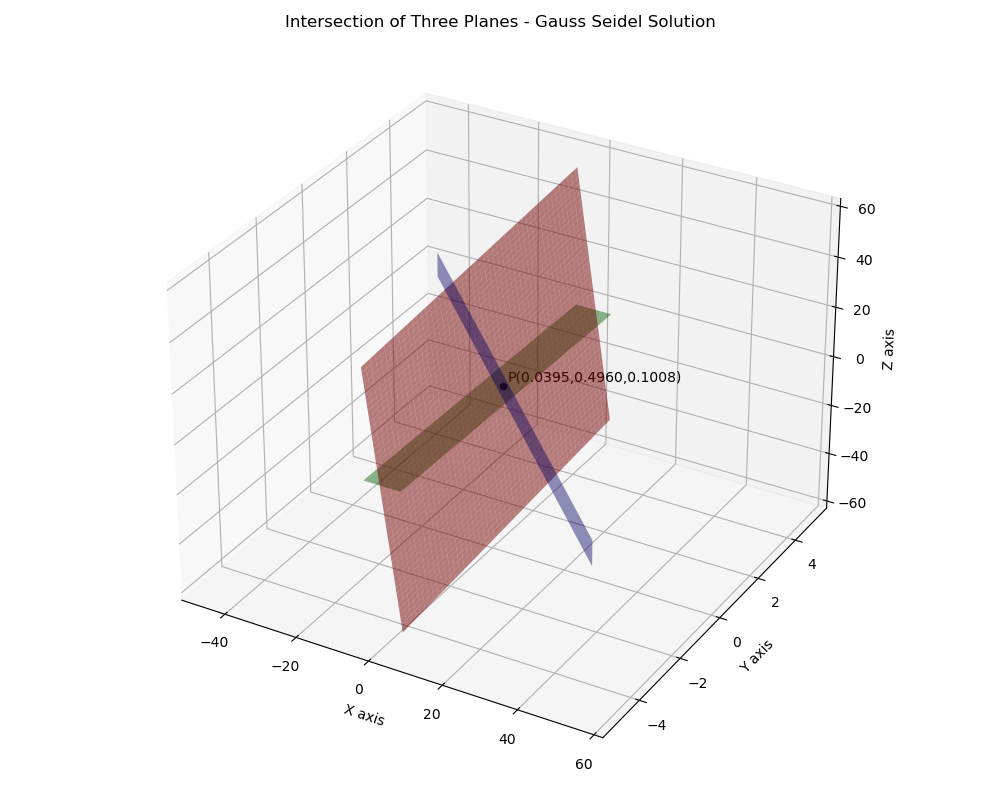
\includegraphics[width=0.7\columnwidth]{figs/solution_gauss_seidel.png} 
   \caption*{Fig : Planes}
  \label{Fig1}
\end{figure}

\end{document}

